\documentclass[11pt, envcountsect, aspectratio=169]{beamer}
\usepackage[utf8]{inputenc}
\usepackage[T1]{fontenc}
\usepackage{lmodern}
\usepackage[english]{babel}
\usepackage{amsmath}
\usepackage{amsfonts}
\usepackage{amssymb}
\usepackage{graphicx}
\usepackage{grffile}
\usetheme{Boadilla}
\usepackage{calrsfs}
\usepackage{nicefrac}
\usepackage{tabularx}

\newenvironment<>{proposition}[1][\undefined]{%
\begin{actionenv}#2%
\ifx#1\undefined%
   \def\insertblocktitle{Theorem}%
\else%
   \def\insertblocktitle{Theorem ({\em#1})}%
\fi%
\par%
\usebeamertemplate{block begin}\em}
{\par\usebeamertemplate{block end}\end{actionenv}}

\definecolor{darkgreen}{rgb}{0.0, 0.2, 0.13}
\definecolor{forestgreen(web)}{rgb}{0.13, 0.55, 0.13}
\definecolor{green(html/cssgreen)}{rgb}{0.0, 0.5, 0.0}

\newcommand{\red}{\textcolor{red}{red}}
\newcommand{\green}{\textcolor{green(html/cssgreen)}{green}}
\newcommand{\blue}{\textcolor{blue}{blue}}

% Subjective Logic macros

\usepackage{calrsfs}

% Domain
\newcommand{\dom}[1]{\mathbb{#1}}

% Powerset
\newcommand{\powset}[1]{\mathcal{P}(\mathbb{#1})}

% Hyperdomain
\newcommand{\hdom}[1]{\mathcal{R}(\mathbb{#1})}

% Composite set
\newcommand{\compset}[1]{\mathcal{C}(\mathbb{#1})}

% Base rate distribution
\newcommand{\ad}[1]{\mathbf{a}_{#1}}
\newcommand{\ada}[2]{\mathbf{a}^{#1}_{#2}}
\newcommand{\adx}[2]{\mathbf{a}_{#1}(#2)}
\newcommand{\adax}[3]{\mathbf{a}^{#1}_{#2}(#3)}

% Belief mass distribution
\newcommand{\bmd}[1]{\mathbf{b}_{#1}}
\newcommand{\bmda}[2]{\mathbf{b}^{#1}_{#2}}
\newcommand{\bmdx}[2]{\mathbf{b}_{#1}(#2)}
\newcommand{\bmdax}[3]{\mathbf{b}^{#1}_{#2}(#3)}

% Uncertainty mass
\newcommand{\ux}[1]{u_{#1}}
\newcommand{\uax}[2]{u^{#1}_{#2}}

% Projected Probability
\newcommand{\ppa}[2]{\mathbf{P}^{#1}_{#2}}

% Opinion
\newcommand{\opi}[1]{\omega_{#1}}
\newcommand{\opia}[2]{\omega^{#1}_{#2}}


\begin{document}

\author{José C. Oliveira}
\title{Subjective Logic}
%\subtitle{}
%\logo{}
%\institute{Universidade Federal de Minas Gerais}
%\date{}
%\subject{}
%\setbeamercovered{transparent}
%\setbeamertemplate{navigation symbols}{}
\begin{frame}[plain]
	\maketitle
\end{frame}

%\section*{Outline}
%\begin{frame}{Summary}
%    \tableofcontents
%\end{frame}

\section{Probabilistic Logic}

\begin{frame}{Probabilistic Logic}
    \begin{figure}
        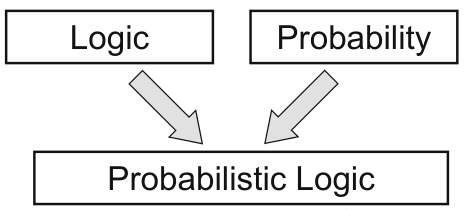
\includegraphics[scale=0.3]{images/probabilistic-logic.png}
    \end{figure}

    \begin{itemize}
        \item It is an extension of binary logic.

        \item Propositions get assigned probabilities.

        \item Formulas of probability calculus replace truth tables.
    \end{itemize}
\end{frame}

\section{Subjective Logic}

\begin{frame}{Subjective Logic}
    \begin{figure}
        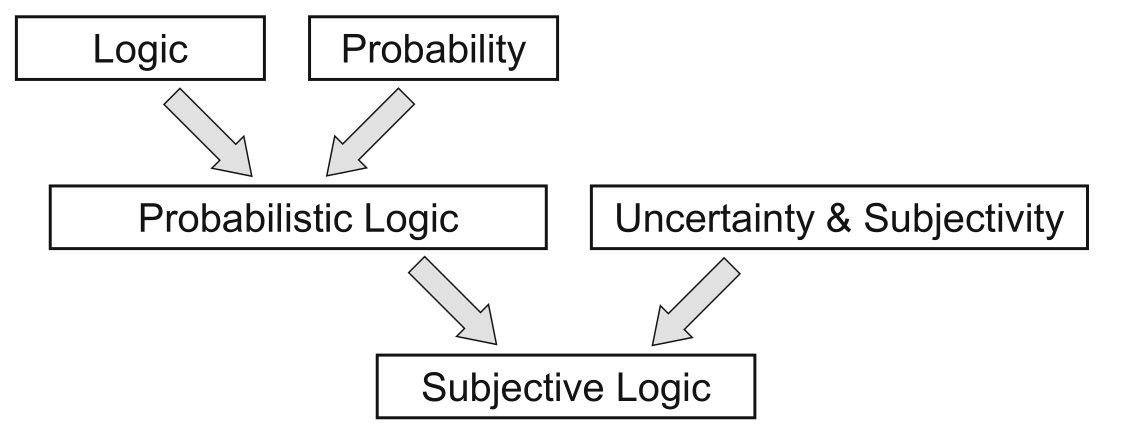
\includegraphics[scale=0.2]{images/subjective-logic.png}
    \end{figure}

    \begin{itemize}
        \item Uncertainty: A \emph{subjetive opinion} can have \emph{uncertainty about probabilities}.

        \item Subjectivity: \emph{Subjective belief ownership} can be explicitly
expressed
    \end{itemize}
\end{frame}

\section{Hyperopinion}

\begin{frame}{Domain}

    \pause

    \begin{definition}
        The \emph{domain} is the set of values that represents possible states (or events) of a variable situation. These events are mutually exclusive.
    \end{definition} ~\\

    \pause

    Suppose we have an urn with balls that can be \red, \green\ or \blue. The domain $\mathbb{X}$ will be:

    \begin{equation}
        \dom{X} = \{\red, \green, \blue\}
    \end{equation}
\end{frame}

\begin{frame}{Hyperdomain}
    \pause

    \begin{definition}
        Let $\dom{X}$ be a domain.\\~\\

        The \emph{hyperdomain} denoted by $\hdom{\dom{X}}$ is

        \begin{equation}
            \text{Hyperdomain: } \hdom{\dom{X}} = \mathcal{P}(\dom{X}) \setminus \{\dom{X}, \emptyset\}
        \end{equation}
    \end{definition} ~\\

    \pause

    The hyperdomain of our urn is:

    \begin{equation}
        \begin{array}{rll}
            \hdom{\dom{X}} = \{ & \{\red\}, \{\green\}, \{\blue\}, \\
            & \{\red, \green\}, \{\red, \blue\}, \{\green, \blue\} & \}
        \end{array}
    \end{equation}

\end{frame}

%\begin{frame}{Base rate distribution}
%    \begin{definition}
%        Let $\dom{X}$ be a domain, and let $X$ be a random variable in $\dom{X}$.\\~\\
%
%        The \emph{base rate distribution} $\ad{X}$ assigns base rate probability to possible
%        values of $X \in \dom{X}$.
%    \end{definition} ~\\
%
%    It is probability distribution used in case we \emph{do not have evidences} about the events, \\a \emph{prior probability}. \\ ~\\
%
%    For all examples, the base rate distribution is uniform.
%\end{frame}

%\begin{frame}{Belief Mass Distribution and Uncertainty Mass}
%    \begin{definition}
%        Let $\dom{X}$ be a domain with corresponding $\hdom{\dom{X}}$, and let $X$ be a hypervariable over $\hdom{\dom{X}}$. \\~\\
%
%        A \emph{belief mass distribution} denoted $\bmd{X}$ assigns belief mass to possible values of the hypervariable $X$.
%    \end{definition} ~\\
%
%    The \emph{belief mass distribution} is subadditive:  $\sum\limits_{x \in \hdom{\dom{X}}} \bmdx{X}{x} \leq 1$.
%
%    The sub-additivity of belief mass distributions is complemented by \emph{uncertainty mass} denoted $\ux{X}$.
%\end{frame}

\begin{frame}{Belief Mass Distribution and Uncertainty Mass}
    \pause

    I told you that our urn has 10 colored balls. One ball is \red, 2 are \blue, and 3 are \green\\ or \blue. Therefore, you know nothing about 4 balls. \\~\\

    \pause

    The belief mass distribution and uncertainty mass will be:

    \begin{equation}
        \begin{array}{ll}
            \bmdx{X}{\{\red\}} & = 0.1 \\
            \bmdx{X}{\{\green\}} & = 0 \\
            \bmdx{X}{\{\blue\}} & = 0.2 \\
            \bmdx{X}{\{\red, \green\}} & = 0 \\
            \bmdx{X}{\{\red, \blue\}} & = 0 \\
            \bmdx{X}{\{\green, \blue\}} & = 0.3 \\
            \ux{X} & = 0.4
        \end{array}
    \end{equation}
\end{frame}

\begin{frame}{Hyper-opinion}
    \pause

    \begin{definition}
        A hyper-opinion on the hypervariable $X$ is the ordered triplet $\opi{X} = \left(\bmd{X}, \ux{X}, \ad{X}\right)$.
    \end{definition} ~\\

    \pause

    The hyper-opinion about our urn is

    \begin{equation}
        \opi{X} = \left(
            \begin{array}{lllll}
                \bmdx{X}{\{\red\}} & = 0.1, & \ & \ad{X} \\
                \bmdx{X}{\{\green\}} & = 0, \\
                \bmdx{X}{\{\blue\}} & = 0.2, \\
                \bmdx{X}{\{\red, \green\}} & = 0, \\
                \bmdx{X}{\{\red, \blue\}} & = 0, \\
                \bmdx{X}{\{\green, \blue\}} & = 0.3, \\
                \ux{X} & = 0.4.
            \end{array}
        \right)
    \end{equation}
\end{frame}

\begin{frame}{Comparison with Dempster-Shafer Belief Theory}
    \pause

    Dempster-Shafer Belief Theory (DST) is a general framework for reasoning with uncertainty.

    \renewcommand{\arraystretch}{1.3}

    \begin{table}[h]
        \begin{tabularx}{\textwidth}{XX}
            \hline
            Dempster-Shafer Belief Theory & Subjective Logic \\ \hline
            DST uses the term ‘frame of discernment’ & SL uses domain. \\
            DST uses \emph{basic belief assignment} denoted by $\mathbf{m}(x)$ & SL uses \emph{belief mass distribution} and \emph{uncertainty mass} \\
            Basic belief can be assigned to the frame & We can't observe evidence about the domain. SL uses uncertainty mass instead. \\
            Dempster’s rule & Belief
            constraint fusion operator. \\
            \hline
        \end{tabularx}
    \end{table}
\end{frame}

%\begin{frame}{Comparison with Imprecise Probabilities}
%    \pause
%
%    In Subjective Logic, an hyperopinion can be represented as a Dirichlet PDF. \\~\\
%
%    \pause
%
%    The Imprecise Dirichlet Model (IDM) is a method for determine upper and lower probabilities produced by setting the minimum and maximum base rates in the Dirichlet PDF. \\~\\
%
%    \pause
%
%    Let $\mathrm{E}^{+}_{X}$ an $\mathrm{E}^{-}_{X}$ be upper and lower probabilities, as defined at the IDM.
%
%    \begin{equation}
%        \ux{X} = \mathrm{E}^{+}_{X} - \mathrm{E}^{-}_{X}
%    \end{equation}
%\end{frame}

\begin{frame}{Comparison with Fuzzy Logic}
    \pause

    In Fuzzy Logic, truth values of variables may be \emph{any real number between 0 and 1}.

    There are levels of truth in the interval that overlaps.

    \pause

    \begin{figure}
        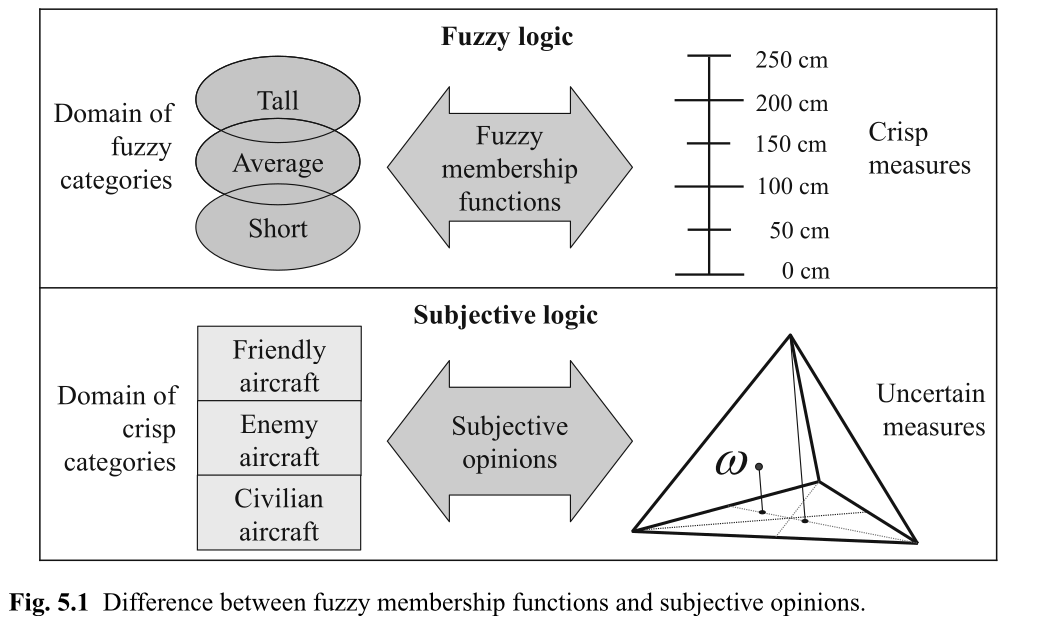
\includegraphics[scale=0.3]{images/fuzzy.png}
    \end{figure}
\end{frame}

\begin{frame}{Comparison with Kleene’s Three-Valued Logic}
    \pause

    Propositions can be assigned one of three truth-values specified as TRUE, FALSE and UNKNOWN.

    \pause

    \begin{equation}
        (x \land y \land \cdots \land z) = \mathrm{UNKNOWN}
    \end{equation} ~\\

    \pause

    In subjective logic, a conjunction of large number of opinions 'I don't know' will say that $(x \land y \land \cdots \land z)$ is likely $\mathrm{FALSE}$.
\end{frame}

%\begin{frame}{Subjective Logic as a Generalisation of Probabilistic Logic}
%    An opinion with $\left|\dom{X}\right| = 2$, all belief mass assigned to one value and no uncertainty is a boolean value. Binary logic applies. \\~\\
%
%    An opinion with no uncertainty is a probability distribution. Probabilistic logic applies.
%\end{frame}

\begin{frame}{What we've done so far}
    \pause

    We studied
    \begin{itemize}
        \item Basic definitions about Subjective Logic
        \item Opinion representations
        \item Decision making
    \end{itemize} ~\\

    \pause

    Next
    \begin{itemize}
        \item Entropy and conflict between opinions
        \item Subjective Logic operators
    \end{itemize}
\end{frame}

\end{document}

